\section{Induction of semantic frames}

\subsection{}

\begin{frame}{FrameNet: frame ``Kidnapping''}

\begin{center}	
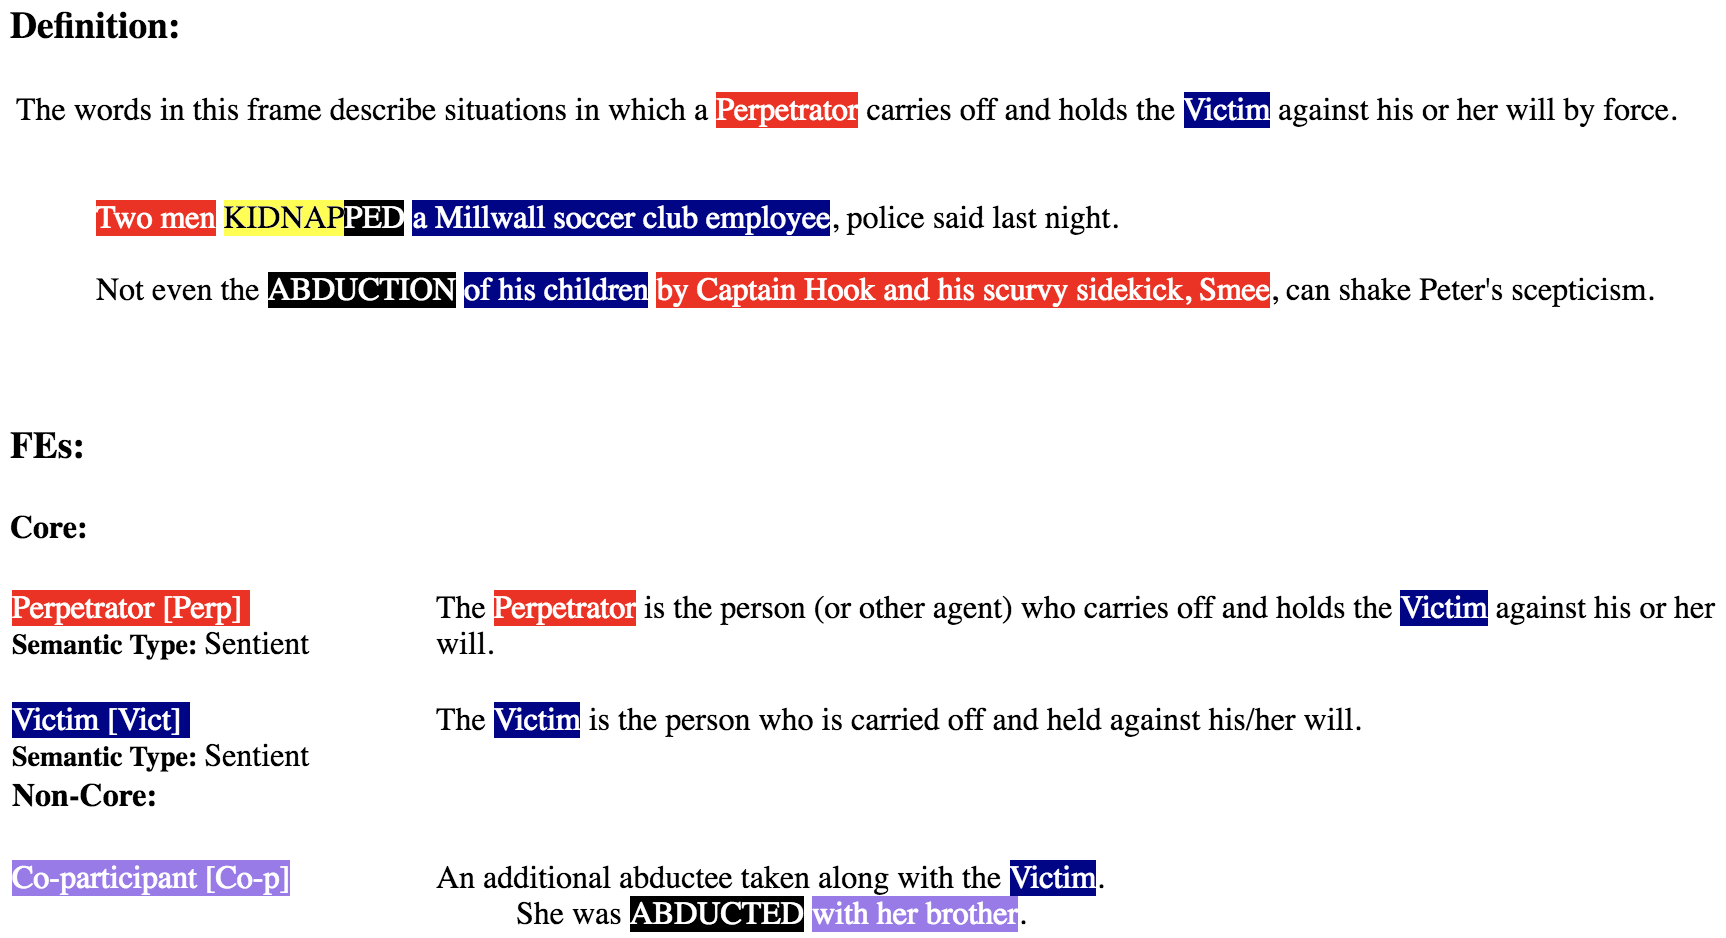
\includegraphics[width=1.0\textwidth]{figures/fn-kidnap}
\end{center}

\end{frame}



\begin{frame}{Frame induction as a triclustering}

\begin{itemize}
\item \textbf{ACL'2018}~\cite{ustalov2018unsupervised}	
\end{itemize}

Example of a LU tricluster corresponding to the ``Kidnapping'' frame from FrameNet.

\begin{table}[t]
\centering
\begin{tabular}{lll}
\textbf{FrameNet~~~~~~~} & \textbf{Role~~~~~~~~} & \textbf{Lexical Units (LU)} \\\toprule
\textit{Perpetrator} & Subject & kidnapper, alien, militant \\ \midrule
\textit{FEE}         & Verb    & snatch, kidnap, abduct \\ \midrule
\textit{Victim}      & Object  & son, people, soldier, child \\
\end{tabular}

\end{table}	

\end{frame}



\begin{frame}{SVO triple elements}


\begin{figure}
  \centering
  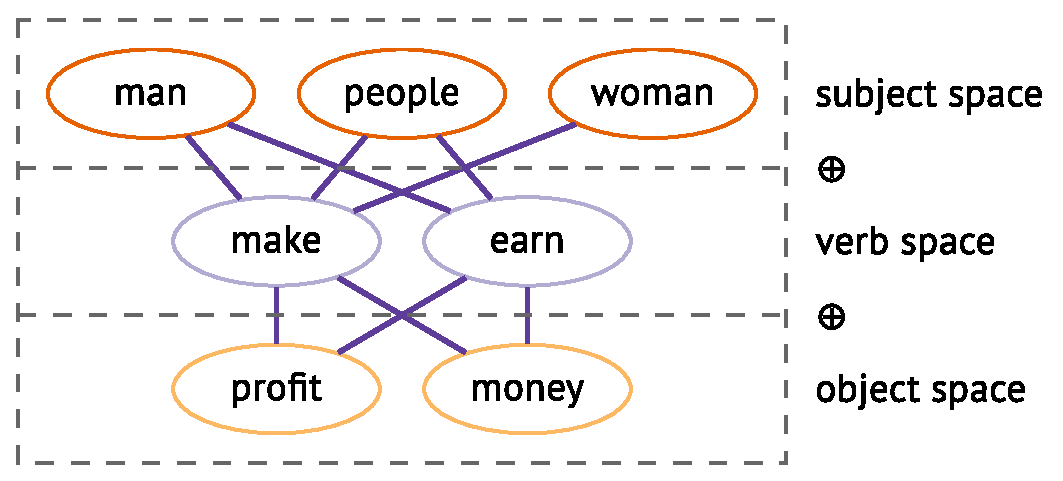
\includegraphics[width=\columnwidth]{figures/triples}
\end{figure}
	
\end{frame}




\begin{frame}{An SVO triple graph}

\vspace{-1em}\begin{figure}
  \centering
  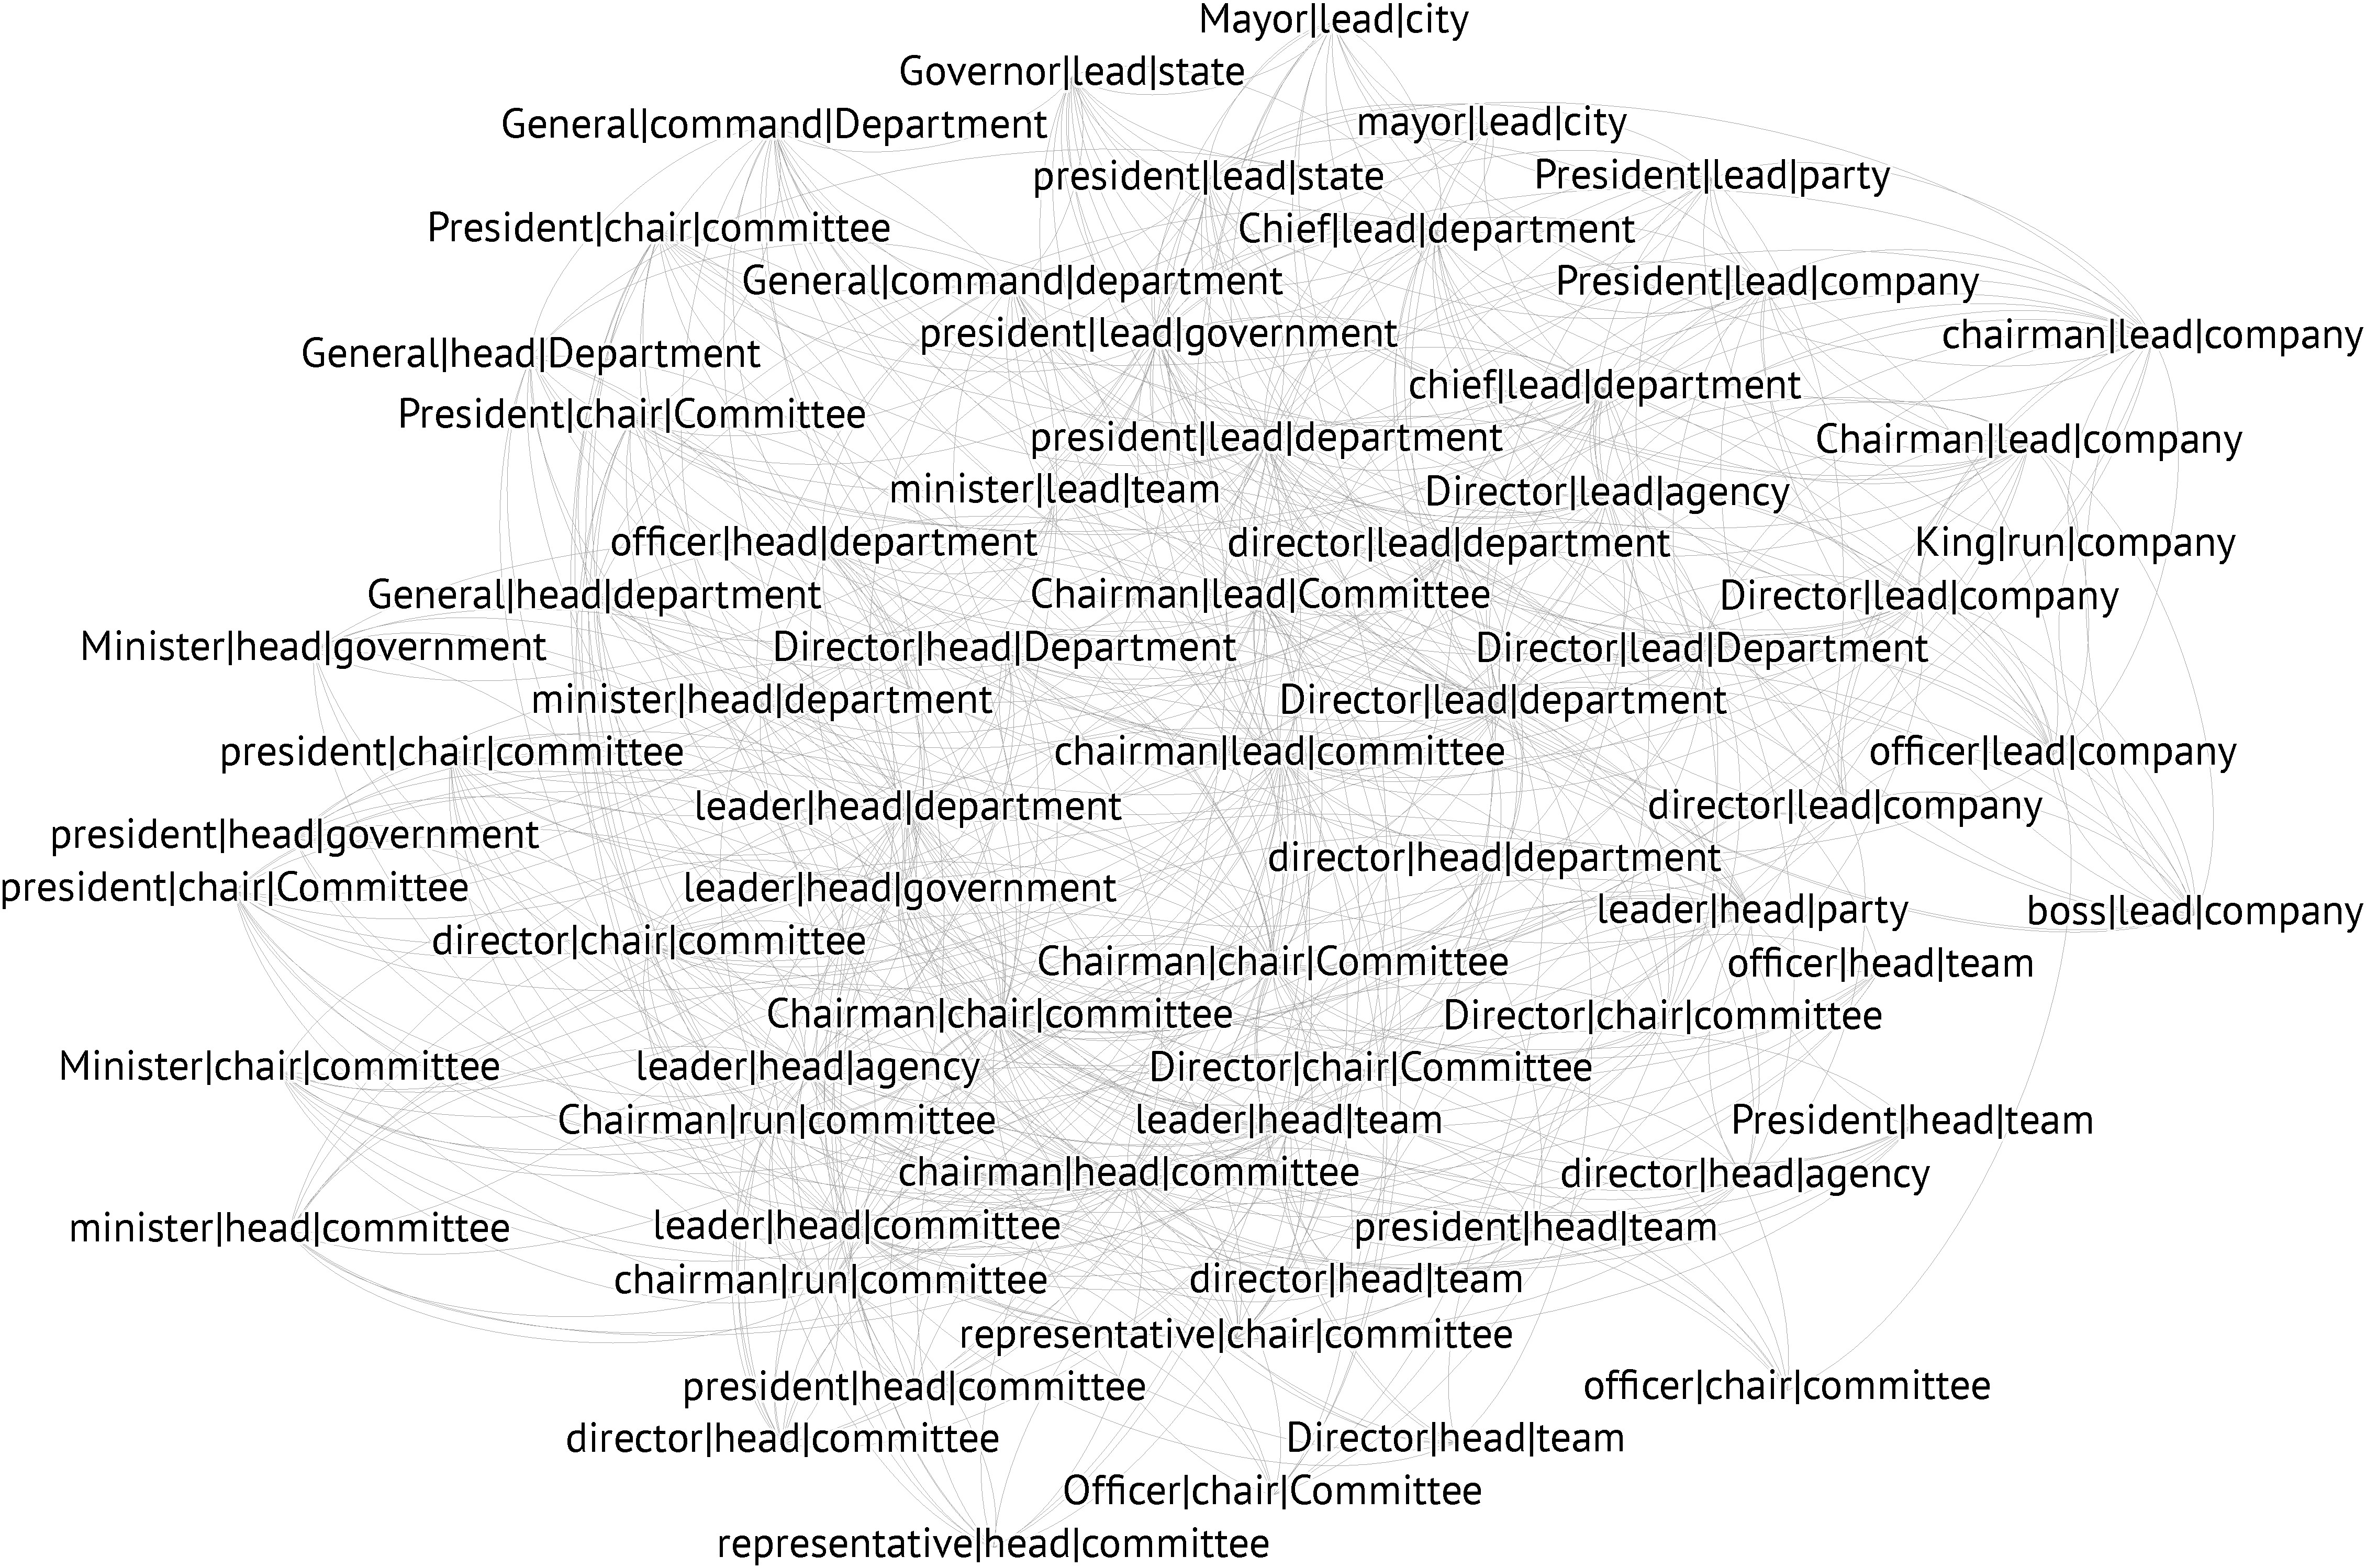
\includegraphics[width=.9\textwidth]{figures/lead}
  
\end{figure}
	
\end{frame}



\begin{frame}{\textit{Triframes} frame induction}

\vspace{-10pt}
\begin{algorithmic}
\REQUIRE{an embedding model $v \in V \rightarrow \vec{v} \in \mathbb{R}^d$,}
\REQUIREP{a set of SVO triples $T \subseteq V^3$,}
\REQUIREP{the number of nearest neighbors $k \in \mathbb{N}$,}
\REQUIREP{a graph clustering algorithm $\textsc{Cluster}$.}
\pause 
\ENSURE{a set of triframes $F$.}
\pause 
\STATE{$S \gets \{t \!\rightarrow \vec{t} \in \mathbb{R}^{3d} : t \in T\}$}
\STATE{$E \gets \{(t, t') \in T^2 : t' \in \NN^S_k(\vec{t}), t \neq t'\}$}
\STATE{$F \gets \emptyset$}
\FORALL{$C \in \textsc{Cluster}(T, E)$}
\STATE{$f_s \gets \{s \in V : (s, v, o) \in C\}$}
\STATE{$f_v \gets \{v \in V : (s, v, o) \in C\}$}
\STATE{$f_o \gets \{o \in V : (s, v, o) \in C\}$}
\STATE{$F \gets F \cup \{(f_s, f_v, f_o)\}$}
\ENDFOR
\RETURN{$F$}
\end{algorithmic}

	
\end{frame}


\begin{frame}{Example of an extracted frame}

\begin{center}
	

  \begin{tabular}{lp{70mm}}\toprule
  \multicolumn{2}{c}{\textbf{Frame \#~848}} \\\toprule
  \textbf{Subjects:} & Company, firm, company \\\midrule
  \textbf{Verbs:}    & buy, supply, discharge, purchase, expect \\\midrule
  \textbf{Objects:}  & book, supply, house, land, share, company, grain, which, item, product, ticket, work, this, equipment, House, it,     film, water, something, she, what, service, plant, time \\\bottomrule
  \end{tabular}
\end{center}
	
\end{frame}


\begin{frame}{Example of an extracted frame}

\begin{figure}
  \centering
  \begin{tabular}{lp{70mm}}\toprule
  \multicolumn{2}{c}{\textbf{Frame \#~849}} \\\toprule
  \textbf{Subjects:} & student, scientist, we, pupil, member, company, man, nobody, you, they, US, group, it, people, Man, user, he          \\\midrule
    \textbf{Verbs:}    & do, test, perform, execute, conduct \\\midrule

  \textbf{Objects:}  & experiment, test \\\bottomrule
  \end{tabular}
\end{figure}
	
\end{frame}




\begin{frame}{Example of an extracted frame}


\begin{figure}[htbp]
  \centering
  \begin{tabular}{lp{70mm}}\toprule
  \multicolumn{2}{c}{\textbf{Frame \#~3207}} \\\toprule
  \textbf{Subjects:} & people, we, they, you \\\midrule
    \textbf{Verbs:}    & feel, seek, look, search \\\midrule

  \textbf{Objects:}  & housing, inspiration, gold, witness, partner, accommodation, Partner \\\bottomrule
  \end{tabular}
\end{figure}


\end{frame}



\begin{frame}{Evaluation datasets}


\begin{tabular}{lrrr}
\textbf{Dataset} & \textbf{\# instances} & \textbf{\# unique} & \textbf{\# clusters} \\\toprule
FrameNet Triples   & 99,744 & 94,170 & 383 \\
Poly. Verb Classes &    246 &    110 & 62 \\
\end{tabular}
	
\end{frame}


\begin{frame}{Evaluation settings}


\begin{tabular}{lrrr}
\textbf{Dataset} & \textbf{\# instances} & \textbf{\# unique} & \textbf{\# clusters} \\\toprule
\textbf{\alert{FrameNet Triples}}   & 99,744 & 94,170 & 383 \\
Poly. Verb Classes &    246 &    110 & 62 \\
\end{tabular}

\pause 

\vspace{20pt}
\textbf{Quality Measures:}

\begin{itemize}
\item $\nmpu$: normalized modified purity, 
\item $\nipu$: normalized inverse purity.	
\end{itemize}

	
\end{frame}



\begin{frame}{Results: comparison to state-of-art}

\begin{center}	
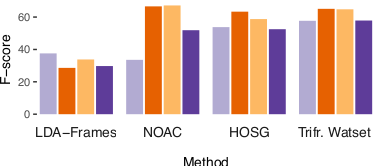
\includegraphics[width=1.0\textwidth]{figures/frames2}
\end{center}


F\textsubscript{1}-scores for \legend{ggplotverb}\,verbs, \legend{ggplotsubject}\,subjects, \legend{ggplotobject}\,objects, \legend{ggplotframe}\,frames

\end{frame}

